\documentclass[../main.tex]{subfiles}
\begin{document}

\section{Resultados}
En este capítulo se presentan los resultados obtenidos tras entrenar, validar y evaluar los modelos desarrollados para la segmentación de lesiones de esclerosis múltiple en imágenes de resonancia magnética. Se analizan tanto los aspectos cuantitativos —mediante métricas estándar de segmentación— como cualitativos, a través de la inspección visual de las predicciones generadas por los modelos.

Los resultados presentados en este capítulo permiten no solo validar el correcto funcionamiento de los modelos implementados, sino también identificar ventajas y limitaciones de cada enfoque en función de la calidad de las segmentaciones obtenidas.


\subsection{Evaluación cuantitativa}
La evaluación cuantitativa tiene como objetivo medir de forma objetiva el rendimiento de los modelos de segmentación utilizando métricas numéricas. Este tipo de evaluación permite comparar de manera rigurosa distintas configuraciones de modelos, arquitecturas y estrategias de preprocesamiento, proporcionando una base sólida para identificar cuáles ofrecen mejores resultados. A diferencia del análisis cualitativo, que se basa en la inspección visual de los resultados, la evaluación cuantitativa facilita una comparación sistemática mediante valores promedio y medidas de dispersión sobre múltiples particiones del conjunto de datos.

En el contexto de la segmentación médica, se han empleado métricas ampliamente aceptadas para cuantificar el grado de coincidencia entre las máscaras generadas por los modelos y las máscaras de referencia creadas por expertos. En concreto, se han utilizado el coeficiente de Dice, el índice de Jaccard (IoU), la precisión y la sensibilidad (recall), cuyas definiciones se recogen en la Sección Metodologías. Para garantizar una evaluación robusta, los resultados se han obtenido mediante validación cruzada con $K=5$ folds, reportando la media y la desviación estándar de cada métrica.

\begin{table}[H]
\centering
\setlength{\tabcolsep}{6pt}
\caption{Resultados medios y desviación estándar de los experimentos (validación cruzada con $K=5$), se marcan en negrita los modelos con DICE más alto de cada configuración.}
\label{tab:resultados_kfold_resumen}
\begin{tabular}{llllcccc}
\toprule
ID &   Red & Selección & SR &   Dice (\%) &   IoU (\%) &   Precisión (\%) &   Recall (\%) \\
\midrule
A & U-Net &     Base & No & 71.07 ± 4.39 & 67.28 ± 3.05 &  72.96 ± 5.76 & 72.09 ± 5.04 \\
B &  YOLO &     Base & No & 71.92 ± 1.58 & 68.81 ± 1.61 &  73.33 ± 1.41 & 72.18 ± 1.93 \\
\textbf{C} & \textbf{U-Net} &     \textbf{Base} & \textbf{x2} & \textbf{73.14 ± 1.64} & \textbf{68.05 ± 1.72} & \textbf{74.13 ± 2.74} & \textbf{75.32 ± 1.08} \\
\textbf{D} &  \textbf{YOLO} &     \textbf{Base} & \textbf{x2} & \textbf{74.60 ± 1.58} & \textbf{71.32 ± 1.49} &  \textbf{76.84 ± 1.38} & \textbf{74.30 ± 1.87} \\
E & U-Net &   Lesión & No & 63.91 ± 3.66 & 51.25 ± 3.90 &  65.40 ± 4.18 & 70.20 ± 3.30 \\
F & U-Net &   Lesión & x2 & 64.68 ± 3.43 & 52.44 ± 3.78 &  68.73 ± 4.43 & 68.18 ± 2.62 \\
G &  YOLO &   Lesión & No & 31.11 ± 6.78 & 23.30 ± 5.40 &  34.33 ± 7.07 & 32.02 ± 6.83 \\
H &  YOLO &   Lesión & x2 & 38.80 ± 7.07 & 30.34 ± 6.00 &  43.74 ± 6.90 & 38.62 ± 7.34 \\
I & U-Net & Cerebro  & No & 67.90 ± 4.12 & 61.76 ± 4.49 &  69.06 ± 4.14 & 70.56 ± 3.93 \\
J & U-Net & Cerebro  & x2 & 72.41 ± 2.19 & 66.34 ± 2.40 &  75.01 ± 3.42 & 73.52 ± 1.31 \\
K &  YOLO & Cerebro  & No & 64.47 ± 2.20 & 60.78 ± 2.57 &  66.22 ± 1.89 & 64.69 ± 2.49 \\
L &  YOLO & Cerebro  & x2 & 67.69 ± 2.58 & 63.72 ± 2.85 &  71.12 ± 1.91 & 66.93 ± 3.14 \\
\bottomrule
\end{tabular}
\end{table}

Los resultados presentados en la Tabla~\ref{tab:resultados_kfold_resumen} muestran cómo el rendimiento de los modelos depende de la estrategia de selección de cortes y de la aplicación de superresolución.  

En la estrategia \textbf{Base}, que incluye los 16.744 cortes (de los cuales 9.994 no presentan lesión y 2.703 son completamente negros), las métricas alcanzan valores altos. Esto se debe a que los cortes sin lesión, que constituyen la mayoría, se contabilizan como predicciones correctas, lo que eleva de forma notable las métricas globales. En este escenario, YOLO obtiene un mejor desempeño (B: 71.92\% Dice) que U-Net (A: 71.07\%), aunque la diferencia es reducida. La aplicación de superresolución aporta una mejora consistente en ambos casos, siendo más pronunciada en YOLO, que alcanza su mejor resultado global con \textbf{74.60\% de Dice (D)}.

La estrategia \textbf{Lesión}, que considera únicamente los 6.750 cortes con lesión, refleja un escenario mucho más exigente, ya que las métricas dependen únicamente de la correcta segmentación de regiones patológicas. Aquí los resultados caen considerablemente: U-Net apenas alcanza 63.91\% de Dice (E), y YOLO baja hasta 31.11\% (G). Incluso aplicando superresolución, las mejoras son limitadas (F: 64.68\% en U-Net y H: 38.80\% en YOLO). Esto sugiere que, sin cortes negativos que aporten contraste, los modelos tienen más dificultades para generalizar y distinguir correctamente entre tejido sano y patológico.

La estrategia \textbf{Cerebro}, que elimina los cortes completamente negros y mantiene un equilibrio entre cortes con y sin lesión (13.563 cortes en total, de los cuales 6.815 no contienen lesión pero sí tejido cerebral visible), ofrece un compromiso intermedio. En este escenario, los modelos disponen de más información anatómica y un balance más realista. U-Net con superresolución alcanza su mejor desempeño con \textbf{72.41\% de Dice (J)}, superando claramente a su configuración Lesión y quedando muy cerca de su resultado en Base. YOLO también mejora respecto a la estrategia Lesión, alcanzando 67.69\% en su mejor configuración (L).

En resumen:
\begin{itemize}
    \item El mejor experimento de \textbf{U-Net} corresponde a la configuración \textbf{Base con SR (C)}, con 73.14\% de Dice.
    \item El mejor experimento de \textbf{YOLO} es la configuración \textbf{Base con SR (D)}, con 74.60\% de Dice.
\end{itemize}

Estas diferencias se explican por la proporción de imágenes en cada estrategia. En Base, la abundancia de cortes sin lesión aumenta las métricas al contarse como correctos, mientras que en Lesión los modelos se enfrentan únicamente al reto de segmentar lesiones, obteniendo valores más bajos. La estrategia Cerebro, al mantener contexto anatómico y cierta proporción de negativos, proporciona un escenario equilibrado y clínicamente más representativo, con resultados competitivos especialmente para U-Net.

En cuanto a precisión, U-Net muestra resultados más elevados, destacando el experimento G con un 76.29\% sin necesidad de superresolución. Curiosamente, al aplicar superresolución (H), la precisión disminuye ligeramente (70.64\%), lo que podría sugerir una ligera sobresegmentación. Por otro lado, YOLO muestra valores más consistentes y moderados, con su mejor resultado en J (66.68\%). Esto sugiere que, si bien YOLO es menos preciso que U-Net en general, tiende a mantener una mayor estabilidad entre experimentos.

Para comprender mejor la correlación entre las proporciones de los cortes y las métricas obtenidas, se presentan distintas figuras que ilustran la distribución de cortes y su impacto en las métricas. La Figura~\ref{fig:proporcion_cortes} muestra la proporción de cortes con y sin lesión de todos los experimentos, destacando cómo la presencia de cortes negativos influye en las métricas globales.

\begin{figure}[!htb]
\minipage{0.32\textwidth}
    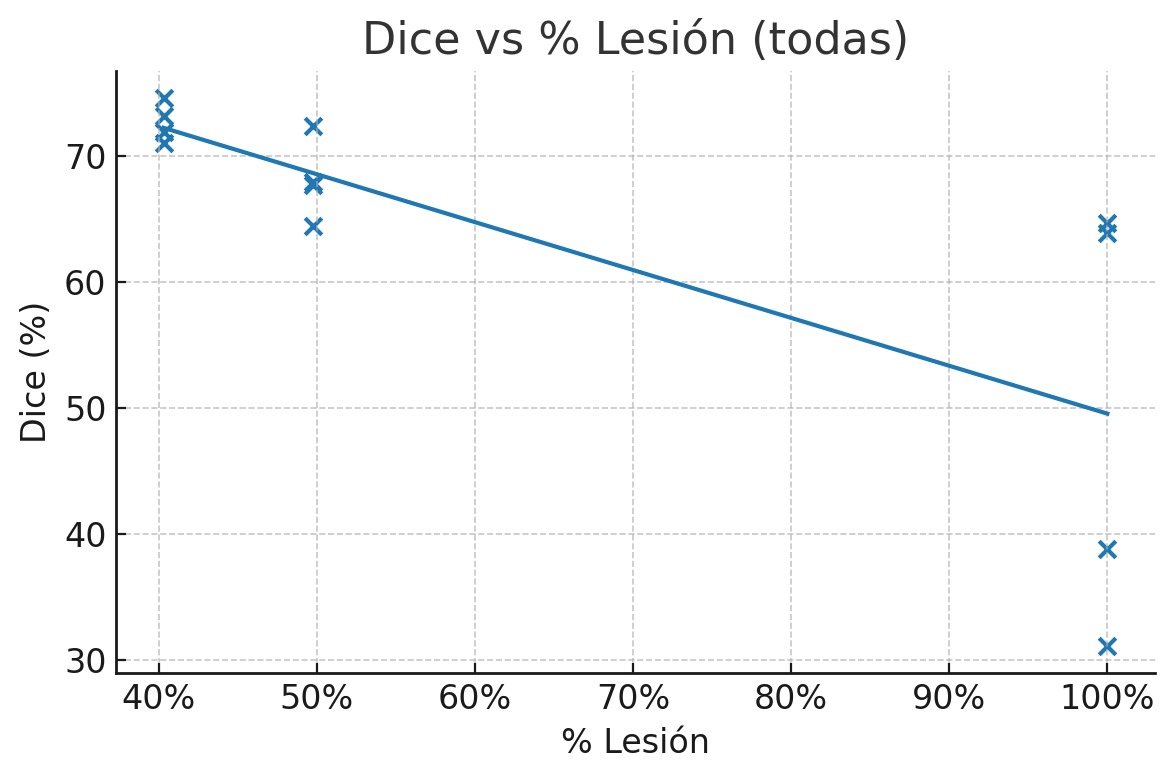
\includegraphics[width=\linewidth]{imgs/resultados/corr/dice_vs_lesion.png}
    \caption{Relación entre Dice y los cortes con lesión.}\label{fig:dice_vs_lesion}
\endminipage\hfill
\minipage{0.32\textwidth}
    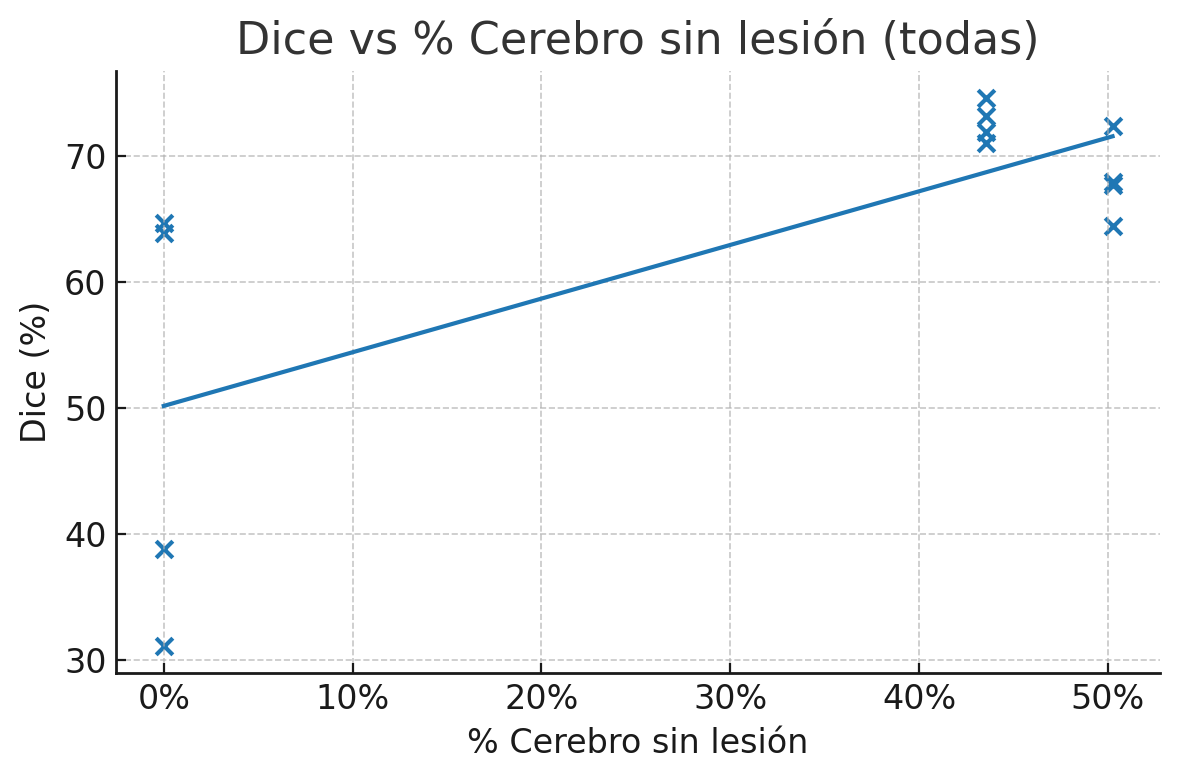
\includegraphics[width=\linewidth]{imgs/resultados/corr/dice_vs_sin_lesion.png}
    \caption{Relación entre Dice y los cortes sin lesión.}\label{fig:dice_vs_sin_lesion}
\endminipage\hfill
\minipage{0.32\textwidth}%
    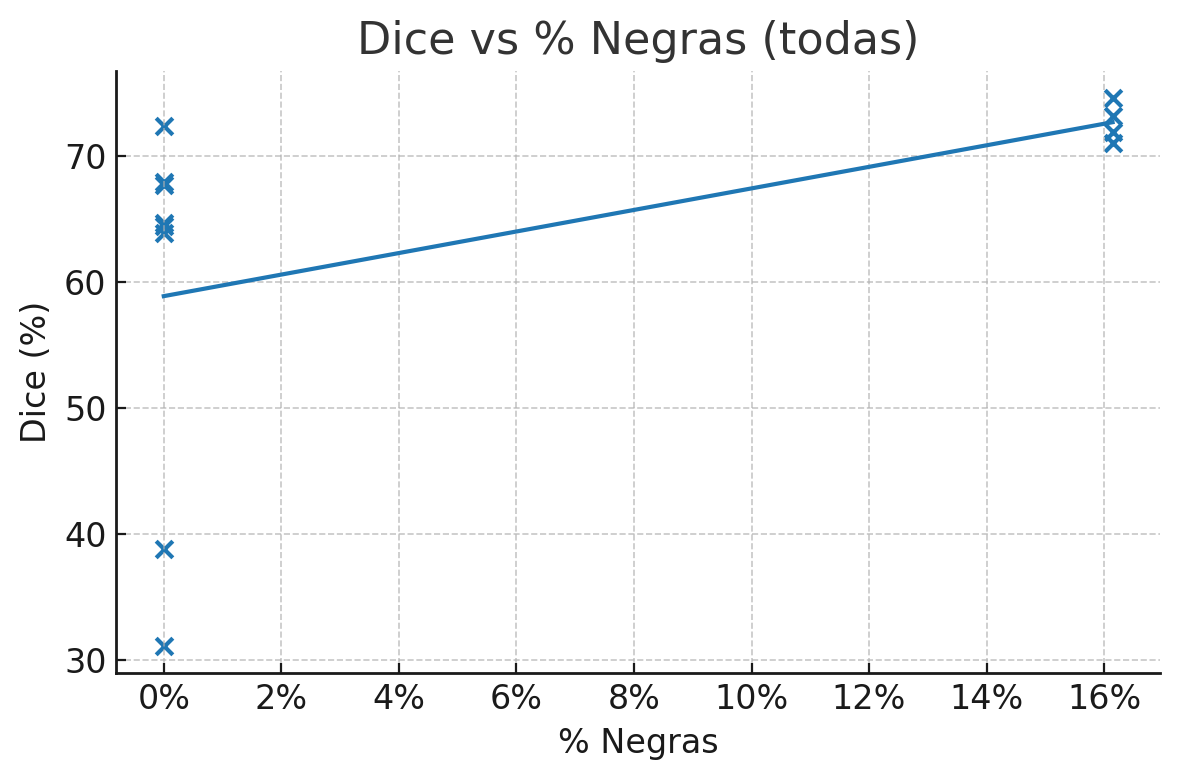
\includegraphics[width=\linewidth]{imgs/resultados/corr/dice_vs_negras.png}
    \caption{Relación entre Dice y los cortes negros.}\label{fig:dice_vs_negras}
\endminipage
\caption{Proporción de cortes con y sin lesión en los experimentos.}
\label{fig:proporcion_cortes}
\end{figure}

Como se observa, las redes disminuyen su rendimiento cuanto mayor proporción de lesión hay, lo que muestra que el desafío es mayor. Contrariamente, cuanta mayor proporción de imágenes negras (es decir, vacías) o sin lesión hay, aumenta el Dice, lo que significa que las redes encuentran fácil predecir cuando no hay lesión, lo que infla las métricas. Por lo tanto, la dificultad está cuanto mayor proporción de cortes con lesión hay. La Figura~\ref{fig:all_dice_vs_lesion} muestra esta conclusión de forma gráfica.

\begin{figure}[H]
    \centering
    \begin{subfigure}[b]{0.48\linewidth}
        \centering
        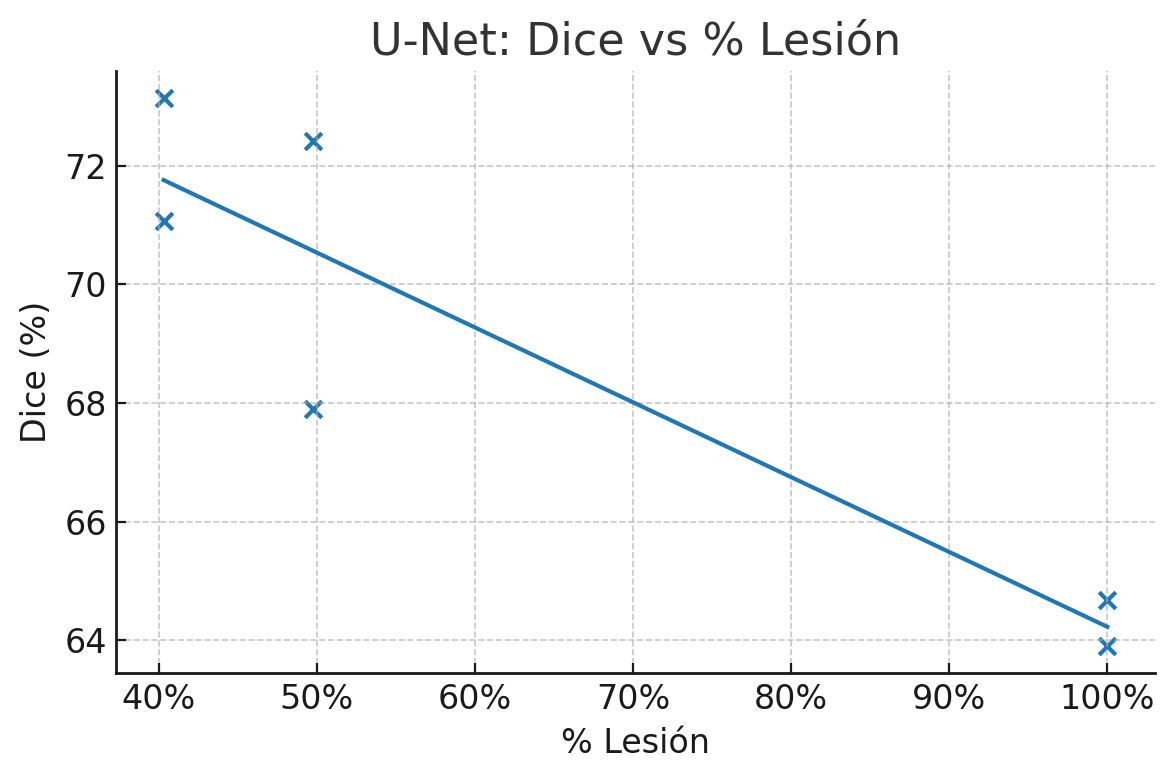
\includegraphics[width=\linewidth]{imgs/resultados/corr/unet_dice_vs_lesion.png}
        \caption{Correlación entre el Dice de la U-Net y la proporción de lesiones.}
        \label{fig:unet_dice_vs_lesion}
    \end{subfigure}
    \hfill
    \begin{subfigure}[b]{0.48\linewidth}
        \centering
        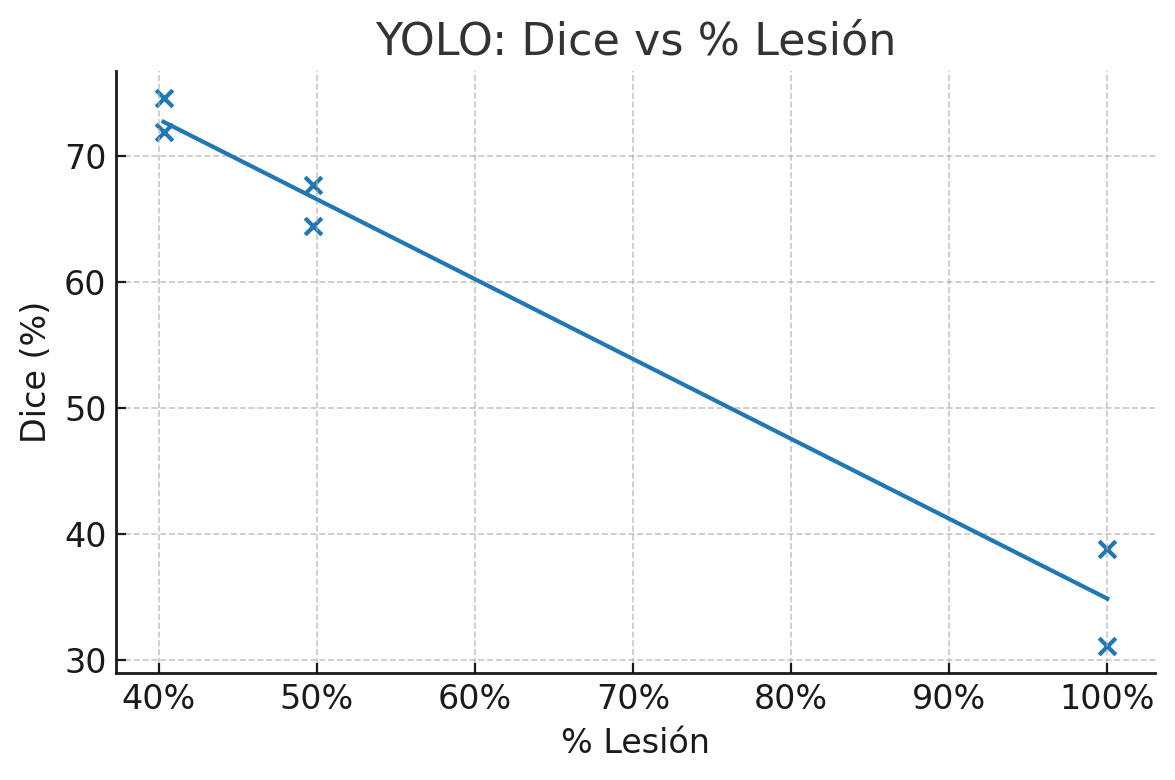
\includegraphics[width=\linewidth]{imgs/resultados/corr/yolo_dice_vs_lesion.png}
        \caption{Correlación entre el Dice de YOLO y la proporción de lesiones.}
        \label{fig:yolo_dice_vs_lesion}
    \end{subfigure}
    \caption{Resumen de la correlación entre Dice y proporción de lesiones.}
    \label{fig:all_dice_vs_lesion}
\end{figure}

La Figura~\ref{fig:heatmap_correlaciones} muestra la relación entre la proporción de los cortes y todas las métricas. Se observa una correlación negativa fuerte entre el porcentaje de cortes con lesión y todas las métricas ($r$ entre –0.67 y –0.86), lo que indica que a medida que aumenta la proporción de cortes positivos el problema se vuelve más exigente y el rendimiento global disminuye. Por el contrario, tanto el porcentaje de cortes sin lesión como el de cortes con cerebro sin lesión presentan correlaciones positivas altas ($r$ entre 0.70 y 0.86), reflejando que disponer de ejemplos negativos con información anatómica facilita al modelo aprender a discriminar y segmentar correctamente. Finalmente, el porcentaje de cortes completamente negros también muestra una correlación positiva moderada ($r \approx 0.45–0.56$), aunque este efecto responde en gran medida a un inflado artificial de las métricas, ya que dichos cortes son triviales de clasificar. En conjunto, el análisis confirma que el equilibrio entre cortes con y sin lesión es determinante para obtener resultados fiables, mientras que un exceso de negativos triviales puede sesgar la evaluación.

\begin{figure}
    \centering
    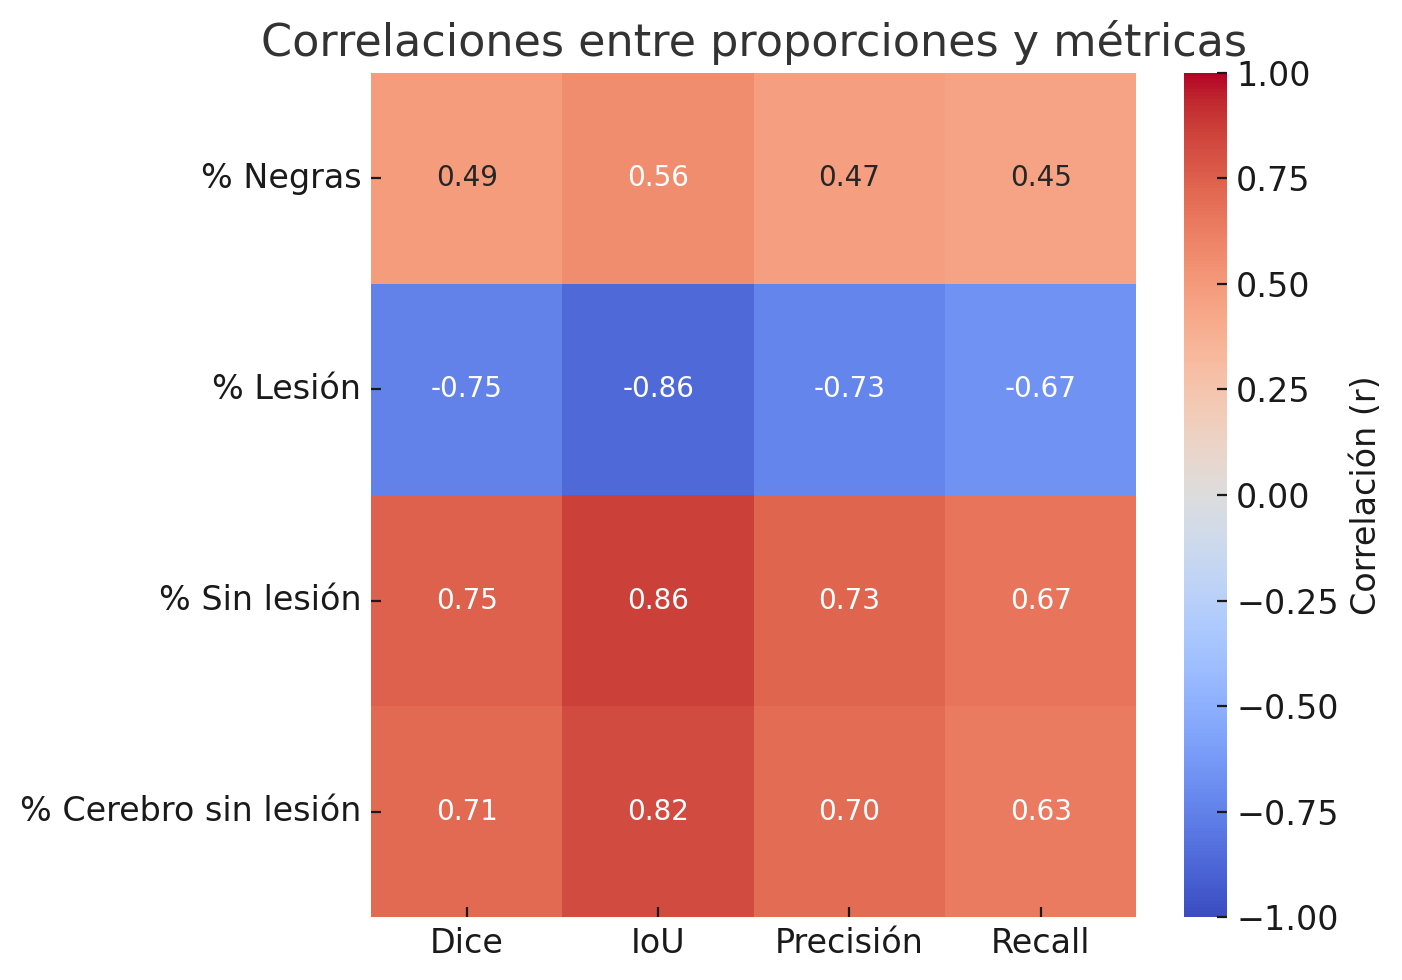
\includegraphics[width=0.8\linewidth]{imgs/resultados/corr/heatmap.png}
    \caption{Mapa de calor de las correlaciones entre proporción de los cortes y métricas obtenidas.}
    \label{fig:heatmap_correlaciones}
\end{figure}

Por otra parte, aunque la aplicación de superresolución puede mejorar las métricas, es importante cuantificar su impacto computacional asociado. Tal como se muestra en la Tabla~\ref{tab:tiempos_inferencia}, el uso de superresolución incrementa los tiempos de inferencia. En el caso de YOLO, aunque la penalización también es evidente, sus tiempos de inferencia siguen siendo considerablemente más bajos que los de U-Net, incluso cuando se aplica superresolución. Esto convierte a YOLO en una opción especialmente atractiva para escenarios donde la velocidad de procesamiento es un requisito crítico, como en entornos clínicos en tiempo real. En definitiva, los resultados muestran que existe un compromiso claro entre precisión y eficiencia, por lo que la elección de una configuración óptima dependerá del contexto de uso y las prioridades del sistema final.

\begin{table}[H]
\centering
\setlength{\tabcolsep}{4pt}
\caption{Tiempo medio de inferencia por imagen y desviación estándar para cada configuración calculado sobre cada fold.}
\label{tab:tiempos_inferencia}
\begin{tabular}{llllc}
\toprule
ID & Red   & Selección  & SR & Tiempo de Inferencia (s) \\
\midrule
A & U-Net & Base         & No  & $2.40 \times 10^{-4} \,\pm\, 7.84 \times 10^{-6}$ \\
B & YOLO  & Base         & No  & $2.09 \times 10^{-2} \,\pm\, 2.34 \times 10^{-3}$ \\
C & U-Net & Base         & x2  & $2.41 \times 10^{-4} \,\pm\, 2.36 \times 10^{-6}$ \\
D & YOLO  & Base         & x2  & $1.22 \times 10^{-2} \,\pm\, 6.00 \times 10^{-4}$ \\
E & U-Net & Lesión       & No  & $2.63 \times 10^{-4} \,\pm\, 1.23 \times 10^{-5}$ \\
F & U-Net & Lesión       & x2  & $1.23 \times 10^{-5} \,\pm\, 2.68 \times 10^{-6}$ \\
G & U-Net & Cerebro      & No  & $2.61 \times 10^{-4} \,\pm\, 1.24 \times 10^{-5}$ \\
H & U-Net & Cerebro      & x2  & $2.90 \times 10^{-4} \,\pm\, 1.30 \times 10^{-5}$ \\
I & YOLO  & Lesión       & No  & $1.94 \times 10^{-2} \,\pm\, 1.70 \times 10^{-3}$ \\
J & YOLO  & Lesión       & x2  & $2.60 \times 10^{-2} \,\pm\, 1.85 \times 10^{-3}$ \\
K & YOLO  & Cerebro      & No  & $1.95 \times 10^{-2} \,\pm\, 2.10 \times 10^{-3}$ \\
L & YOLO  & Cerebro      & x2  & $1.71 \times 10^{-2} \,\pm\, 4.21 \times 10^{-3}$ \\
\bottomrule
\end{tabular}
\end{table}

\subsection{Evaluación cualitativa}
Con el objetivo de complementar la evaluación cuantitativa y analizar la calidad visual de las segmentaciones generadas por los modelos, se ha llevado a cabo un análisis cualitativo sobre una muestra representativa del conjunto de test. Esta evaluación permite observar el comportamiento de los modelos ante diferentes escenarios clínicos, como lesiones pequeñas, múltiples o con bordes difusos, aspectos que pueden no ser capturados adecuadamente mediante métricas numéricas.

A continuación se muestran algunos ejemplos de predicción considerados clínicamente relevantes de cada modelo entrenado por experimento y por red. Empezando por la Figura~\ref{fig:P1_T1_Z105_matriz_12exps}, que muestra al paciente 1, punto temporal T1 y corte número 105. En este caso, la U-Net supera claramente a YOLO, logrando una segmentación más precisa y completa de la lesión principal, así como de las pequeñas lesiones adyacentes, aunque ha tenido un falso positivo en una pequeña lesión en la parte inferior. 

\begin{figure}[H]
    \centering
    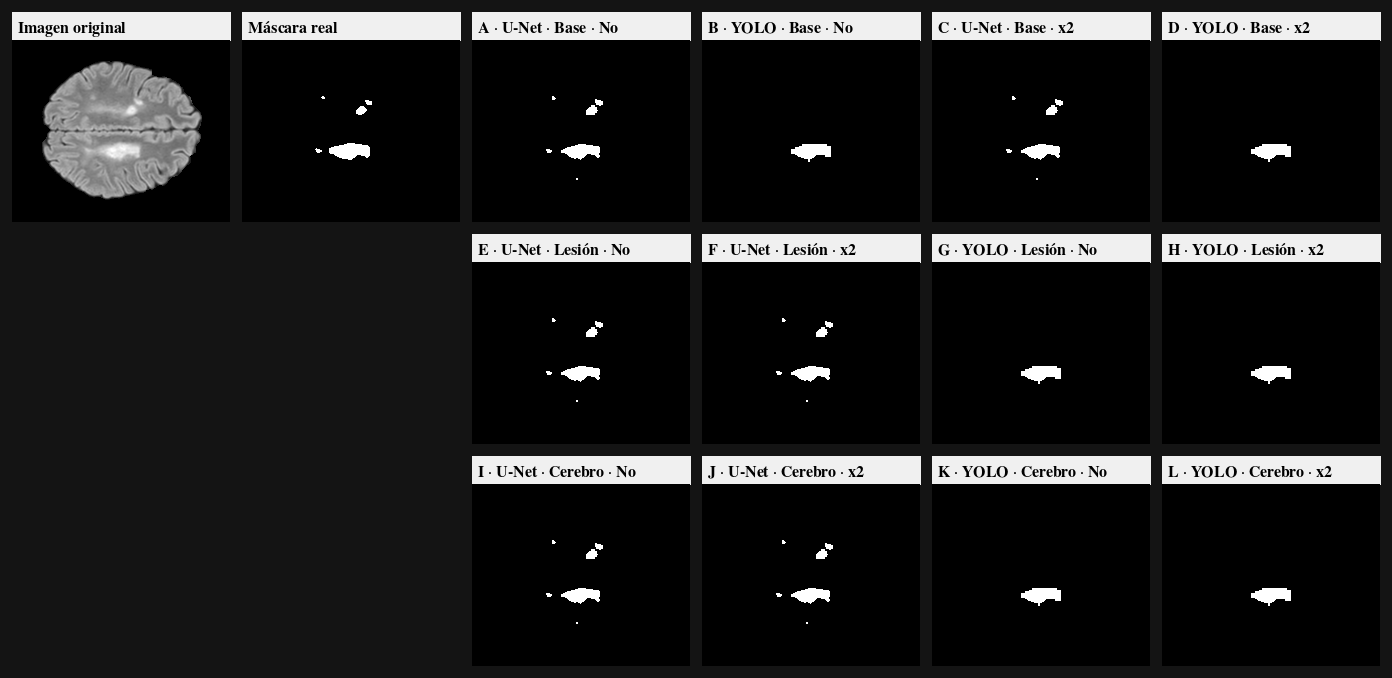
\includegraphics[width=1\linewidth]{imgs/resultados/comp/P1_T1_Z105_matriz_12exps.png}
    \caption{Lesión grande con cuatro lesiones pequeñas alrededor.}
    \label{fig:P1_T1_Z105_matriz_12exps}
\end{figure}

La Figura~\ref{fig:P12_T4_Z105_matriz_12exps} corresponde a una lesión pequeña bien delimitada del paciente 12, punto temporal T4 y corte número 105. En este caso, U-Net y YOLO logran una localización precisa. Puede verse claramente la predicción por polígonos de YOLO, que capta la lesión como un área cuadrada, mientras que U-Net ofrece una segmentación más detallada y ajustada a la forma real de la lesión. 

\begin{figure}[H]
    \centering
    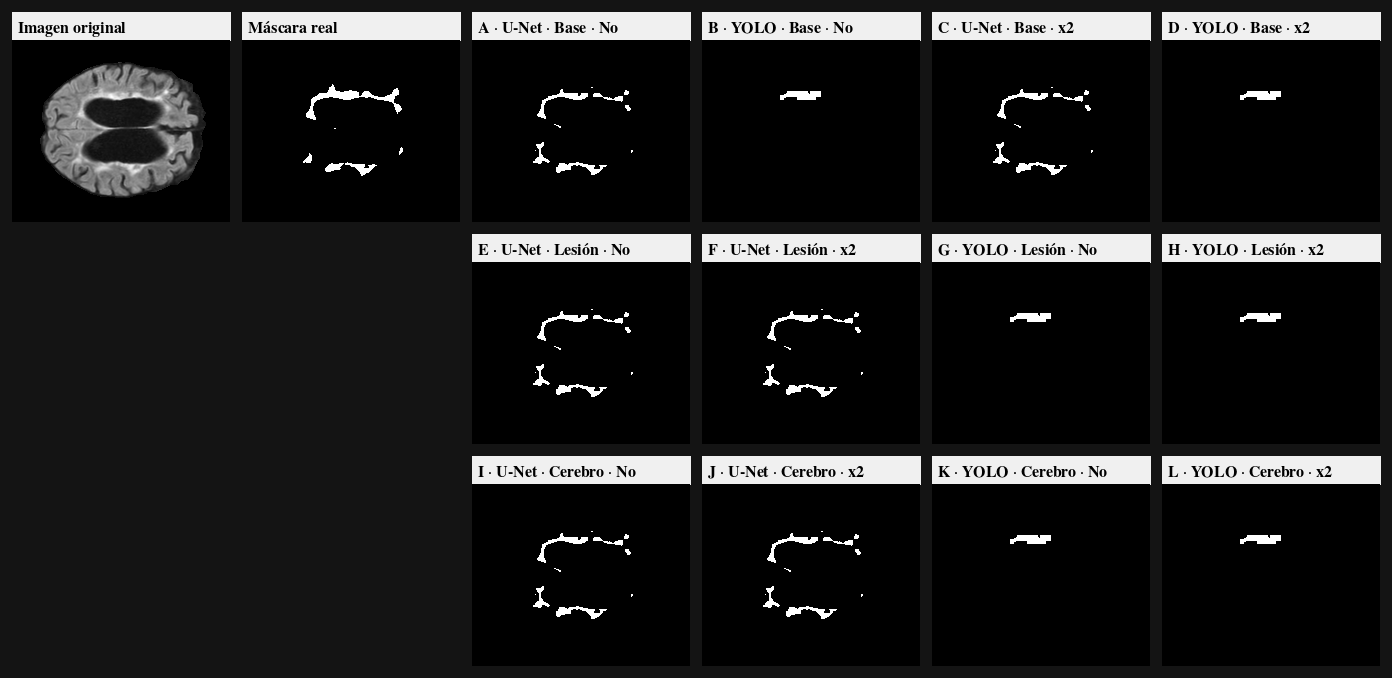
\includegraphics[width=1\linewidth]{imgs/resultados/comp/P12_T4_Z105_matriz_12exps.png}
    \caption{Lesión pequeña bien delimitada. U-Net ofrece una predicción muy precisa; YOLO comete un falso positivo en una región sin lesión.}
    \label{fig:P12_T4_Z105_matriz_12exps}
\end{figure}

La Figura~\ref{fig:P10_T2_Z100_matriz_12exps} representa una lesión fragmentada con áreas pequeñas y dispersas, paciente 10, punto temporal T2 y corte número 100. En este caso, U-Net logra una segmentación ligeramente muy buena aunque no perfecto. La YOLO no logra captar ninguna lesión.

\begin{figure}[H]
    \centering
    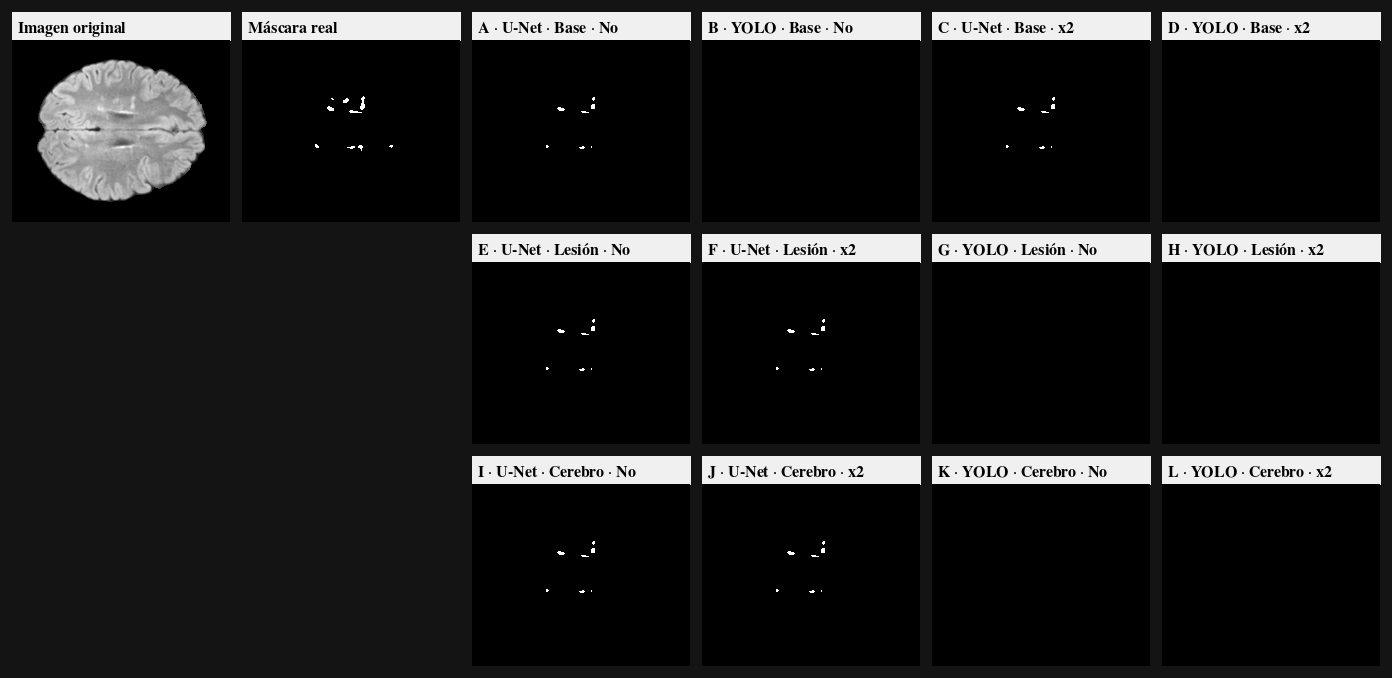
\includegraphics[width=1\linewidth]{imgs/resultados/comp/P10_T2_Z100_matriz_12exps.png}
    \caption{Lesión extensa alrededor del centro cerebral. U-Net sobresegmenta ligeramente, mientras YOLO no logra abarcar toda el área.}
    \label{fig:P10_T2_Z100_matriz_12exps}
\end{figure}

La Figura \ref{fig:P33_T2_Z98_matriz_12exps} muestra una lesión compleja repartida en áreas con regiones circulares, paciente 33, punto temporal T2 y corte número 98. La U-Net logra segmentar de manera más completa aunque con falsos positivos y ligera sobresegmentación. YOLO no es capaz de captar la lesión en su totalidad, presentando un solo área que no corresponde con la realidad.

\begin{figure}[H]
    \centering
    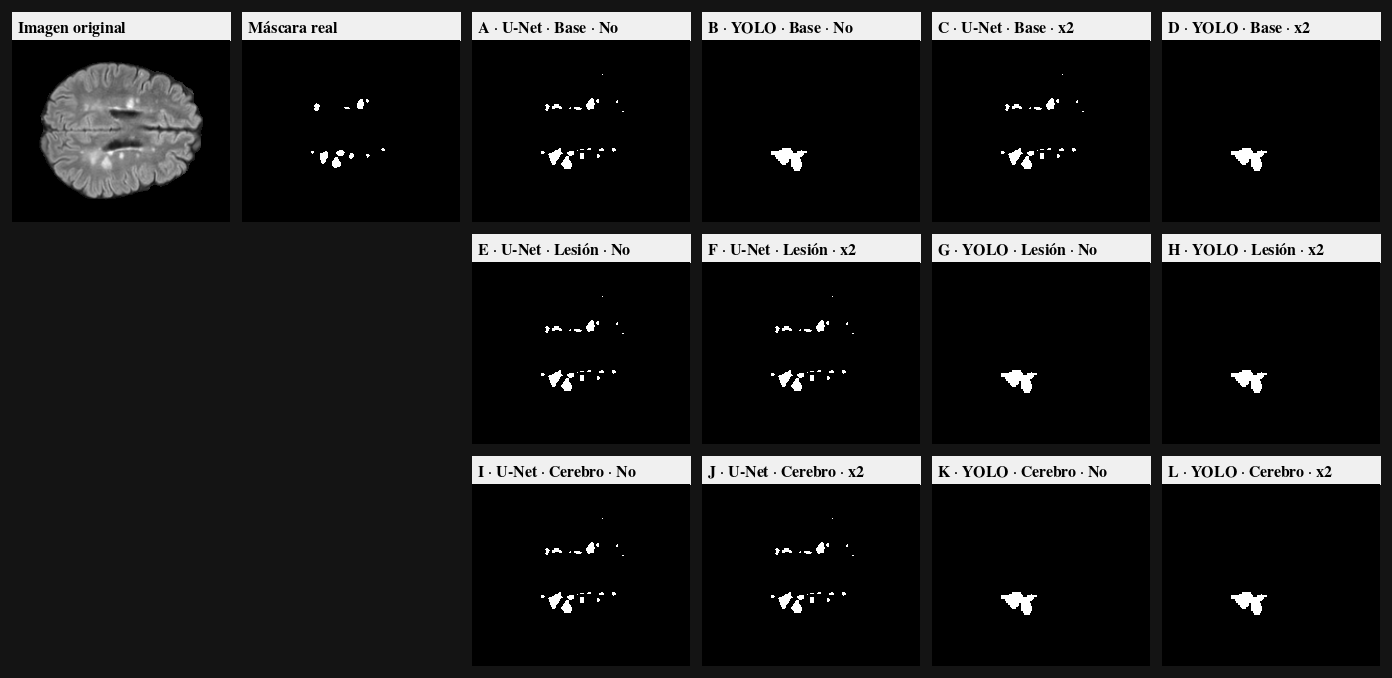
\includegraphics[width=1\linewidth]{imgs/resultados/comp/P33_T2_Z98_matriz_12exps.png}
    \caption{Lesiones fragmentadas y dispersas. YOLO solo capta un área mayor que la máscara real.}
    \label{fig:P33_T2_Z98_matriz_12exps}
\end{figure}

%-----------------------------------------------------------------
La Figura \ref{fig:P7_T1_Z99_matriz_12exps} representa una lesión dividida en dos partes, paciente 7, punto temporal T1 y corte número 99. En este caso, tanto U-Net como YOLO logran identificar las dos áreas lesionadas. Sin embargo, U-Net ofrece una segmentación más detallada y precisa, capturando mejor los bordes irregulares de las lesiones, mientras que YOLO presenta una segmentación más simplificada y menos ajustada.

\begin{figure}[H]
    \centering
    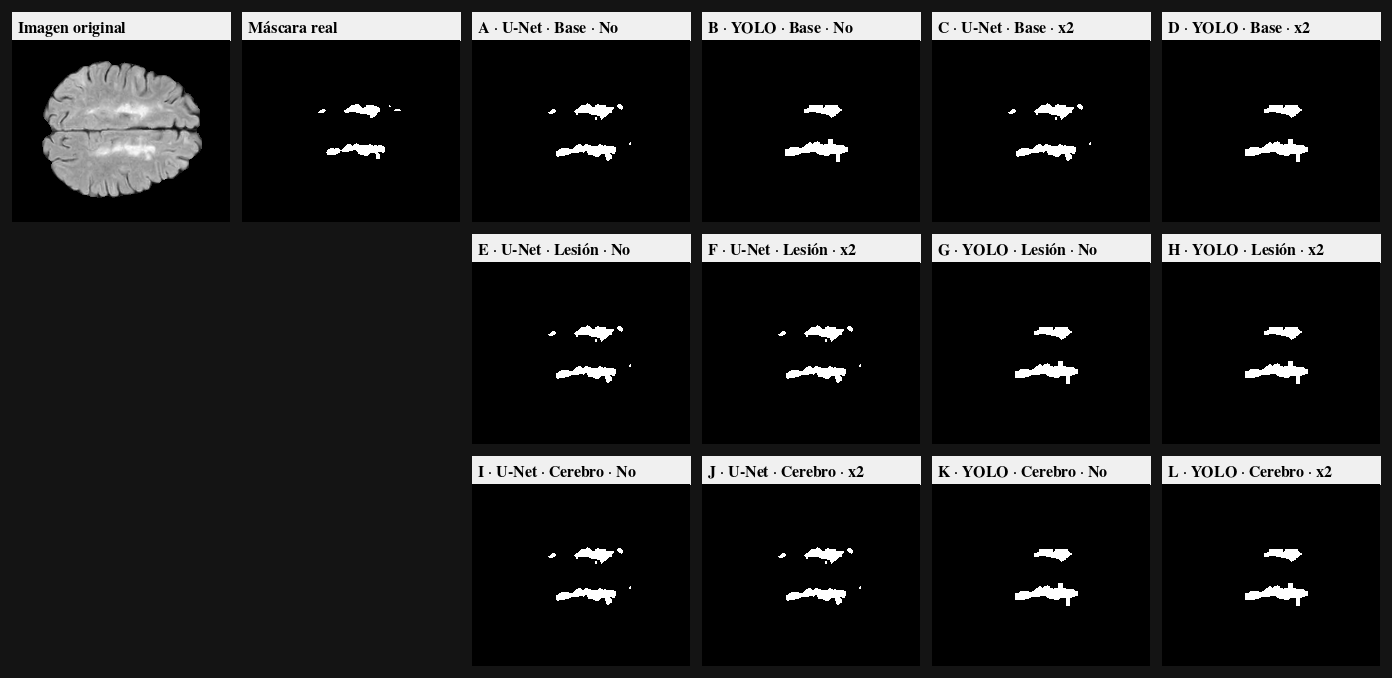
\includegraphics[width=1\linewidth]{imgs/resultados/comp/P7_T1_Z99_matriz_12exps.png}
    \caption{Lesión en dos áreas separadas. U-Net proporciona una segmentación más detallada, mientras YOLO ofrece una representación más simplificada.}
    \label{fig:P7_T1_Z99_matriz_12exps}
\end{figure}


\end{document}